\documentclass[11pt, a4paper]{report}

% --- CODIFICACIÓN, IDIOMA Y TIPOGRAFÍA ---
% Compilar con XeLaTeX o LuaLaTeX (compatible con MiKTeX local y Overleaf)
\usepackage{fontspec}
\usepackage[english, spanish]{babel}
\IfFileExists{C:/Windows/Fonts/segoeui.ttf}{
    \setmainfont{Segoe UI}
    \setsansfont{Segoe UI}
    \setmonofont{Consolas}
}{
    \setmainfont{Noto Sans}
    \setsansfont{Noto Sans}
    \setmonofont{Noto Sans Mono}
}
\renewcommand{\familydefault}{\sfdefault}

% --- MÁRGENES Y GEOMETRÍA ---
\usepackage[
    a4paper,
    top=2.5cm,
    bottom=2.5cm,
    left=2.5cm,
    right=2.5cm,
    headheight=22pt
]{geometry}

% --- PALETA DE COLORES FINTECH / BANCA INSTITUCIONAL ---
\usepackage[table]{xcolor}
\definecolor{NavyPrimary}{HTML}{081C3F}    % Azul medianoche (dominante)
\definecolor{CyanAccent}{HTML}{0077B6}     % Azul técnico (acento)
\definecolor{SlateText}{HTML}{1E293B}      % Gris carbón para lectura cómoda
\definecolor{MutedGray}{HTML}{64748B}      % Gris pizarra para metadatos y pies
\definecolor{LightTint}{HTML}{F1F5F9}      % Fondo sutil para tablas y cajas

% --- MATEMÁTICAS, TABLAS, CÓDIGO Y GRÁFICOS ---
\usepackage{amsmath, amssymb}
\usepackage{booktabs}
\usepackage{array}
\usepackage{tabularx}
\usepackage{longtable}
\usepackage{graphicx}
\graphicspath{{figures/}{../../img/}}
\usepackage{float}
\usepackage{subcaption}
\usepackage[font=small, labelfont={bf, color=NavyPrimary}, textfont={color=MutedGray}]{caption}
\usepackage{csquotes}
\usepackage[most]{tcolorbox}
\usepackage{listings}

% --- ESTILO DE BLOQUES DE CÓDIGO ---
\lstset{
    basicstyle=\ttfamily\small\color{SlateText},
    backgroundcolor=\color{LightTint},
    frame=leftline,
    framerule=2pt,
    rulecolor=\color{CyanAccent},
    breaklines=true,
    showstringspaces=false,
    aboveskip=1em,
    belowskip=1em,
    xleftmargin=0.8em,
    framexleftmargin=0.5em
}

% --- CAJAS DESTACADAS (PREGUNTA DE INVESTIGACIÓN, ADRS, HALLAZGOS) ---
\newtcolorbox{cajadestacada}[1][]{
    enhanced,
    breakable,
    colback=LightTint,
    colframe=LightTint,
    borderline west={3pt}{0pt}{CyanAccent},
    coltitle=NavyPrimary,
    fonttitle=\bfseries\small,
    title={#1},
    boxrule=0pt,
    arc=2pt,
    left=10pt,
    right=10pt,
    top=8pt,
    bottom=8pt,
    before skip=1em,
    after skip=1em
}

% --- BIBLIOGRAFÍA (BibLaTeX + Biber) ---
\usepackage[backend=biber, style=ieee, sorting=none]{biblatex}
\addbibresource{referencias.bib}

% --- CABECERAS, PIES Y LISTAS ---
\usepackage{fancyhdr}
\usepackage{enumitem}
\setlist[itemize]{label=\textcolor{CyanAccent}{\textbullet}, leftmargin=1.5em}
\setlist[enumerate]{label=\textcolor{NavyPrimary}{\textbf{\arabic*.}}, leftmargin=1.5em}

% --- ENLACES Y METADATOS PDF ---
\usepackage{hyperref}
\hypersetup{
    colorlinks=true,
    linkcolor=NavyPrimary,
    citecolor=CyanAccent,
    urlcolor=CyanAccent,
    pdftitle={Motor Predictivo Hibrido de Mercados Financieros - TFM},
    pdfauthor={Arturo Carrillo Jimenez, Felipe Tais Diaz}
}

% --- ESTILO DE PÁGINA INTERIOR ---
\pagestyle{fancy}
\fancyhf{}
\fancyhead[L]{\footnotesize\color{MutedGray}\textsc{Motor Predictivo Híbrido de Mercados Financieros (US Big 6)}}
\fancyhead[R]{\footnotesize\color{MutedGray}\thepage}
\renewcommand{\headrulewidth}{0.4pt}
\renewcommand{\headrule}{\hbox to\headwidth{\color{LightTint}\leaders\hrule height \headrulewidth\hfill}}

\fancypagestyle{plain}{
    \fancyhf{}
    \fancyfoot[R]{\footnotesize\color{MutedGray}\thepage}
    \renewcommand{\headrulewidth}{0pt}
}

% --- ESTILO DE CAPÍTULOS Y SECCIONES ---
\makeatletter
\def\@makechapterhead#1{%
  \vspace*{20\p@}%
  {\parindent \z@ \raggedright \normalfont
    \ifnum \c@secnumdepth >\m@ne
        \fontsize{11}{13}\selectfont\bfseries\color{CyanAccent}
        \MakeUppercase{\@chapapp\ \thechapter}
        \par\nobreak
        \vskip 6\p@
    \fi
    \interlinepenalty\@M
    \fontsize{22}{26}\selectfont\bfseries\color{NavyPrimary} #1\par\nobreak
    \vskip 10\p@
    {\color{NavyPrimary}\hrule height 1.2pt}
    \vskip 24\p@
  }}
\def\@makeschapterhead#1{%
  \vspace*{20\p@}%
  {\parindent \z@ \raggedright
    \normalfont
    \interlinepenalty\@M
    \fontsize{22}{26}\selectfont\bfseries\color{NavyPrimary} #1\par\nobreak
    \vskip 10\p@
    {\color{NavyPrimary}\hrule height 1.2pt}
    \vskip 24\p@
  }}
\makeatother

\color{SlateText}
\setlength{\parindent}{0pt}
\setlength{\parskip}{0.65em}
\linespread{1.15}
\emergencystretch=1.8em

\begin{document}

% ==============================================================================
% PORTADA ESTILO INFORME FINTECH / BANCA INSTITUCIONAL
% ==============================================================================
\begin{titlepage}
    \thispagestyle{empty}
    \noindent
    \begin{minipage}[t]{0.5\textwidth}
        \raggedright
        {\fontsize{13}{15}\selectfont\bfseries\color{NavyPrimary} EBIS} {\fontsize{10}{12}\selectfont\color{MutedGray} Business Techschool}
    \end{minipage}%
    \begin{minipage}[t]{0.5\textwidth}
        \raggedleft
        {\fontsize{9}{11}\selectfont\color{MutedGray} Universidad de Vitoria-Gasteiz} {\fontsize{13}{15}\selectfont\bfseries\color{NavyPrimary} EUNEIZ}
    \end{minipage}

    \vspace{2.8cm}

    {\fontsize{9.5}{12}\selectfont\bfseries\color{CyanAccent}
    TRABAJO FIN DE MÁSTER \quad $\cdot$ \quad MÁSTER EN DATA SCIENCE E INTELIGENCIA ARTIFICIAL}

    \vspace{0.5cm}

    {\fontsize{26}{32}\selectfont\bfseries\color{NavyPrimary}\raggedright
    Motor Predictivo Híbrido de\\Mercados Financieros\par}

    \vspace{0.4cm}

    {\fontsize{13}{18}\selectfont\color{MutedGray}
    Arquitectura integral de ingesta multimodal, alineación temporal Point-in-Time y regresión cuantílica sobre el universo bancario estadounidense (US Big 6)\par}

    \vspace{1.2cm}
    {\color{CyanAccent}\rule{3.5cm}{2pt}}
    \vspace{1.5cm}

    % Bloque de metadatos con barra lateral institucional
    \begin{tabular}{!{\color{NavyPrimary}\vrule width 2.5pt}l l}
        \textbf{\color{NavyPrimary}Autores:} & Arturo Carrillo Jiménez $\cdot$ Felipe Tais Díaz \\[0.4em]
        \textbf{\color{NavyPrimary}Tutor:} & Germán Cubas Guillé \\[0.4em]
        \textbf{\color{NavyPrimary}Universo de estudio:} & JPM $\cdot$ BAC $\cdot$ WFC $\cdot$ C $\cdot$ GS $\cdot$ MS (2010--2023) \\[0.4em]
        \textbf{\color{NavyPrimary}Fecha de entrega:} & Febrero de 2027 \\
    \end{tabular}

    \vfill

    % Franja inferior minimalista con indicadores técnicos del proyecto
    {\color{LightTint}\hrule height 1pt}
    \vspace{0.4cm}
    {\footnotesize\color{MutedGray}
    \textbf{STACK \& METODOLOGÍA:} Medallion Architecture (Bronze / Silver / Gold) $\cdot$ NLP Gatekeeper \& Sentiment (LLM / FinBERT) $\cdot$ Point-in-Time Alignment $\cdot$ Quantile Regression}
\end{titlepage}

% ==============================================================================
% RESUMEN EJECUTIVO (1 PÁGINA INDEPENDIENTE ANTES DEL ÍNDICE — REQUISITO EBIS)
% ==============================================================================
\chapter*{Resumen ejecutivo}
\addcontentsline{toc}{chapter}{Resumen ejecutivo}

\textit{[Espacio reservado para el Resumen Ejecutivo de 1 página. Se redactará al finalizar la fase experimental para sintetizar el problema de negocio, la arquitectura multimodal, las métricas de calibración cuantílica obtenidas y el impacto en gestión de riesgo.]}

\vspace{1em}
\noindent\textbf{\color{NavyPrimary}Palabras clave:} Finanzas cuantitativas, procesamiento de lenguaje natural financiero, FinBERT, modelos de lenguaje, alineación temporal Point-in-Time, regresión cuantílica, arquitectura Medallion, US Big 6.

\clearpage

% ==============================================================================
% ÍNDICES (MÁXIMO 60 PÁGINAS TOTALES SEGÚN NORMATIVA EBIS)
% ==============================================================================
\tableofcontents
% \listoffigures
% \listoftables
\clearpage

% ==============================================================================
% CAPÍTULOS MODULARES
% ==============================================================================
\chapter{Introducción}

\section{Contexto y motivación del problema}
La modelización cuantitativa de los mercados financieros ha estado tradicionalmente dominada por el análisis técnico clásico y por enfoques estadísticos basados exclusivamente en series temporales endógenas. No obstante, en entornos caracterizados por una elevada liquidez y exposición informativa constante, la dinámica de los activos responde de forma asimétrica a flujos de información exógena no estructurada, tales como comunicados corporativos, eventos regulatorios, informes de analistas y noticias macroeconómicas.

El presente Trabajo Fin de Máster (TFM) acota su estudio al universo bancario sistémico estadounidense, conocido como el \textbf{US Big 6}: JPMorgan Chase \& Co. (\texttt{JPM}), Bank of America Corp. (\texttt{BAC}), Wells Fargo \& Co. (\texttt{WFC}), Citigroup Inc. (\texttt{C}), The Goldman Sachs Group, Inc. (\texttt{GS}) y Morgan Stanley (\texttt{MS}). Este conjunto de entidades constituye un laboratorio idóneo por su alta profundidad de mercado, su sensibilidad a decisiones de política monetaria y la densidad de cobertura mediática que reciben diariamente.

\begin{cajadestacada}[Pregunta central de investigación]
\textit{«¿Podemos anticipar cambios de tendencia o picos de volatilidad en las acciones de los gigantes bancarios de EE.UU. combinando el histórico de precios con el tono de las noticias y eventos regulatorios antes de la apertura del mercado (09:30 AM ET)?»}
\end{cajadestacada}

Respecto al planteamiento inicial recogido en la propuesta del proyecto, el desarrollo empírico ha motivado una evolución arquitectónica sustancial. En lugar de depender de una única fuente histórica estática o de aplicar modelos de lenguaje directamente sobre textos sin depurar, el sistema se ha reestructurado hacia una \textbf{arquitectura multimodal e incremental} basada en el patrón \textit{Medallion} (\textit{Bronze}, \textit{Silver} y \textit{Gold}). Esta separación permite auditar sistemáticamente la calidad del dato crudo, aislar múltiples vectores de contaminación semántica y garantizar la trazabilidad completa entre cada evento informativo y su impacto sobre la sesión bursátil correspondiente.

\section{Planteamiento del problema y justificación metodológica}
El diseño de sistemas predictivos robustos en finanzas exige superar cuatro fallos metodológicos recurrentes en la literatura aplicada:

\begin{enumerate}
    \item \textbf{No estacionariedad de los precios absolutos:} El entrenamiento directo sobre niveles de precios introduce correlaciones espurias y degrada la capacidad de generalización fuera de muestra. Para mitigar este efecto, la formulación del problema se traslada al dominio de los retornos logarítmicos continuos ($r_{t+1} = \ln(C_{t+1}/C_t)$) y medidas de dispersión condicional.
    \item \textbf{Sesgo de mirada al futuro (\textit{Look-Ahead Bias}):} La integración ingenua de noticias y precios suele asumir disponibilidad instantánea de la información, contaminando el conjunto de entrenamiento con señales posteriores al instante de decisión. Para erradicar esta fuga de información, se implementa una alineación temporal estricta \textit{Point-in-Time} (PiT) sincronizada con el calendario operativo de la Bolsa de Nueva York (NYSE).
    \item \textbf{Ruido semántico y discontinuidad de mercado cerrado:} Los flujos de noticias financieras presentan duplicidades, colisiones de \textit{tickers} (por ejemplo, \texttt{GS} o \texttt{MS} dentro de palabras comunes), menciones periféricas en artículos multisujeto y sesgos derivados de revisiones de \textit{analyst ratings}. Asimismo, la acumulación de eventos durante fines de semana, festivos o registros sin hora exacta (\texttt{date\_only}) requiere un tratamiento específico alineado con las sesiones de mercado (\texttt{premarket}, \texttt{intraday}, \texttt{afterhours} y desplazamiento conservador a $t+1$).
    \item \textbf{Insuficiencia de la predicción puntual:} Estimar únicamente el valor esperado de un retorno oculta la incertidumbre inherente al régimen de volatilidad vigente. La adopción de \textbf{regresión cuantílica} permite estimar bandas condicionales de probabilidad (cuantiles $q=0.10$ y $q=0.90$ para un intervalo empírico del 80\,\%), proporcionando una herramienta directamente accionable para la gestión de riesgo y el dimensionamiento de coberturas pre-apertura.
\end{enumerate}

\section{Objetivos del TFM}
\subsection*{Objetivo general}
Diseñar, implementar y validar un motor predictivo híbrido y multimodal para el universo bancario \textit{US Big 6} que integre series temporales cuantitativas con señales de sentimiento financiero depuradas, operando bajo una alineación temporal \textit{Point-in-Time} y un enfoque de regresión cuantílica para la estimación de rangos de retorno y riesgo.

\subsection*{Objetivos específicos}
\begin{itemize}
    \item \textbf{OE1. Ingeniería de datos en capas:} Construir un pipeline reproducible estructurado bajo el patrón \textit{Medallion} (\textit{Bronze}, \textit{Silver} y \textit{Gold}) que integre series de mercado ajustadas, eventos regulatorios oficiales (SEC EDGAR) y corpus históricos y en vivo de noticias financieras.
    \item \textbf{OE2. Auditoría y depuración semántica (Quality Gate):} Desarrollar un protocolo de filtrado mediante procesamiento de lenguaje natural para resolver colisiones de entidades, desduplicar registros, aislar contextos relevantes por entidad y neutralizar ruido fuera de dominio y \textit{analyst ratings}.
    \item \textbf{OE3. Sincronización temporal Point-in-Time:} Implementar un motor de cruce temporal acoplado al calendario bursátil estadounidense (\texttt{America/New\_York}) que garantice ausencia total de fuga de información futura y modele adecuadamente los bloques de mercado cerrado.
    \item \textbf{OE4. Modelado cuantílico multimodal:} Entrenar y calibrar modelos de regresión cuantílica capaces de estimar intervalos condicionales de retorno al 80\,\% de cobertura empírica para los seis activos del universo \textit{US Big 6}.
    \item \textbf{OE5. Validación comparativa, explicabilidad y visualización:} Evaluar el desempeño mediante métricas de calibración de intervalos (\textit{Pinball Loss}, \textit{Winkler Score}) y estudios de ablación (modelo cuantitativo puro frente a modelo híbrido), complementando los resultados con explicabilidad (TreeSHAP) y un cuadro de mando operativo.
\end{itemize}

\section{Alcance y estructura de la memoria}
El alcance de este trabajo comprende el diseño arquitectónico completo, la auditoría exploratoria de datos, la implementación de los pipelines de transformación y modelado, la validación estadística mediante particionado temporal estricto y la exposición de resultados a través de un cuadro de mando analítico en Streamlit. Quedan fuera del alcance la ejecución automatizada de órdenes en mercados reales (\textit{live execution}) y el modelado de microestructura de alta frecuencia (\textit{tick-by-tick}), los cuales se plantean como líneas futuras de evolución.

La memoria se organiza en los siguientes capítulos:
\begin{itemize}
    \item \textbf{Capítulo 2 (Estado del Arte):} Revisión crítica de la literatura sobre análisis de sentimiento financiero, fusión multimodal de datos y modelado cuantílico en series temporales.
    \item \textbf{Capítulo 3 (Arquitectura del Sistema, Modelo de Datos e Ingesta):} Descripción separada de la infraestructura \textit{Medallion} en Cloudflare R2, el modelo y estructura de datos por capa, las fuentes \textit{Bronze}, la arquitectura \textit{Clean} y el cumplimiento normativo.
    \item \textbf{Capítulo 4 (Auditoría Exploratoria y Capa Silver):} Diagnóstico cuantitativo de ruido en capa \textit{Bronze}, funcionamiento del \textit{Gatekeeper} semántico, extracción de sentimiento y alineación \textit{Point-in-Time}.
    \item \textbf{Capítulo 5 (Ingeniería de Características y Modelado):} Construcción de variables técnicas y cualitativas, selección con Boruta, formulación de regresión cuantílica y protocolo de validación temporal.
    \item \textbf{Capítulo 6 (Experimentos, Resultados y Explicabilidad):} Evaluación de calibración de intervalos, estudio de ablación, análisis TreeSHAP y simulación de gestión de riesgo.
    \item \textbf{Capítulo 7 (Despliegue y Visualización):} Orquestación productiva, aseguramiento de calidad (tests y análisis estático) e interfaz analítica desarrollada.
    \item \textbf{Capítulo 8 (Conclusiones, Impacto y Líneas Futuras):} Síntesis de hallazgos, análisis de impacto económico/operativo (ROI) y trabajos futuros.
\end{itemize}

\chapter{Estado del Arte}

\section{Procesamiento de lenguaje natural en el dominio financiero}
El vocabulario financiero presenta ambigüedades semánticas que invalidan los diccionarios y modelos de propósito general. Como demostraron Loughran y McDonald~\cite{loughran2011liability}, términos habituales en informes corporativos (como \textit{liability}, \textit{tax} o \textit{exposure}) se clasifican erróneamente como negativos en léxicos genéricos de sentimiento.

Para superar esta limitación, la literatura reciente ha convergido hacia modelos basados en arquitectura \textit{Transformer} preentrenados sobre corpus económicos y regulatorios, destacando \textbf{FinBERT}~\cite{yang2020finbert}. Estudios posteriores como el de Lopez-Lira y Tang~\cite{lopezlira2023chatgpt} han demostrado asimismo el potencial de los modelos de lenguaje de gran escala (LLM) para anticipar retornos diarios a partir de titulares financieros, planteando un equilibrio clave entre precisión semántica, latencia y coste computacional en producción.

\section{Fusión multimodal y rigor temporal en finanzas}
La combinación de series temporales de precios con flujos textuales dispersos fue formalizada en trabajos de referencia como StockNet~\cite{xu2018stock}. Sin embargo, el éxito práctico de estos enfoques depende del rigor en la validación temporal para evitar fugas de información (\textit{data leakage}) y correlaciones seriales espurias~\cite{lopezdeprado2018advances, jansen2020ml}.

\section{Regresión cuantílica y explicabilidad (XAI)}
\textit{[Completar: fundamentar la transición desde clasificación binaria / regresión a la media hacia regresión cuantílica con Pinball Loss para modelar volatilidad condicional e incertidumbre, así como el uso de TreeSHAP para auditar la atribución de variables textuales frente a indicadores técnicos.]}

\section{Brecha identificada y contribución del TFM}
\textit{[Completar: resumir en tabla comparativa qué aporta este TFM frente a enfoques habituales (Gatekeeper Few-Shot + SEC 8-K + Anexos EX-* + Point-in-Time NYSE + Regresión Cuantílica al 80\,\% + arquitectura Always Free).]}

\chapter{Arquitectura del Sistema e Ingesta (Capa Bronze)}

\section{Arquitectura Cloud Always Free y patrón Medallion}
El sistema ha sido diseñado bajo una premisa de coste operativo nulo en almacenamiento y análisis (\textit{Always Free}), evitando tarifas de transferencia (\textit{egress}) mediante \textbf{Cloudflare R2} (compatible con la API S3 Signature v4) y aplicando la arquitectura \textbf{Medallion}:

\begin{itemize}
    \item \textbf{Capa Bronze (\texttt{raw/}):} Datos inmutables en formato columnar Parquet con compresión \texttt{ZSTD} (y artefactos crudos preservados con esquema en lectura).
    \item \textbf{Capa Silver (\texttt{silver/}):} Registros depurados, normalizados al huso horario \texttt{America/New\_York}, filtrados por el \textit{Gatekeeper} semántico y enriquecidos con puntuaciones de sentimiento.
    \item \textbf{Capa Gold (\texttt{gold/}):} Matrices tabulares unificadas $(X_t \rightarrow y_{t+1})$ listas para entrenamiento, inferencia y consumo desde el cuadro de mando.
\end{itemize}

% Ejemplo para insertar el diagrama de arquitectura cuando se copie a figures/
% \begin{figure}[H]
%     \centering
%     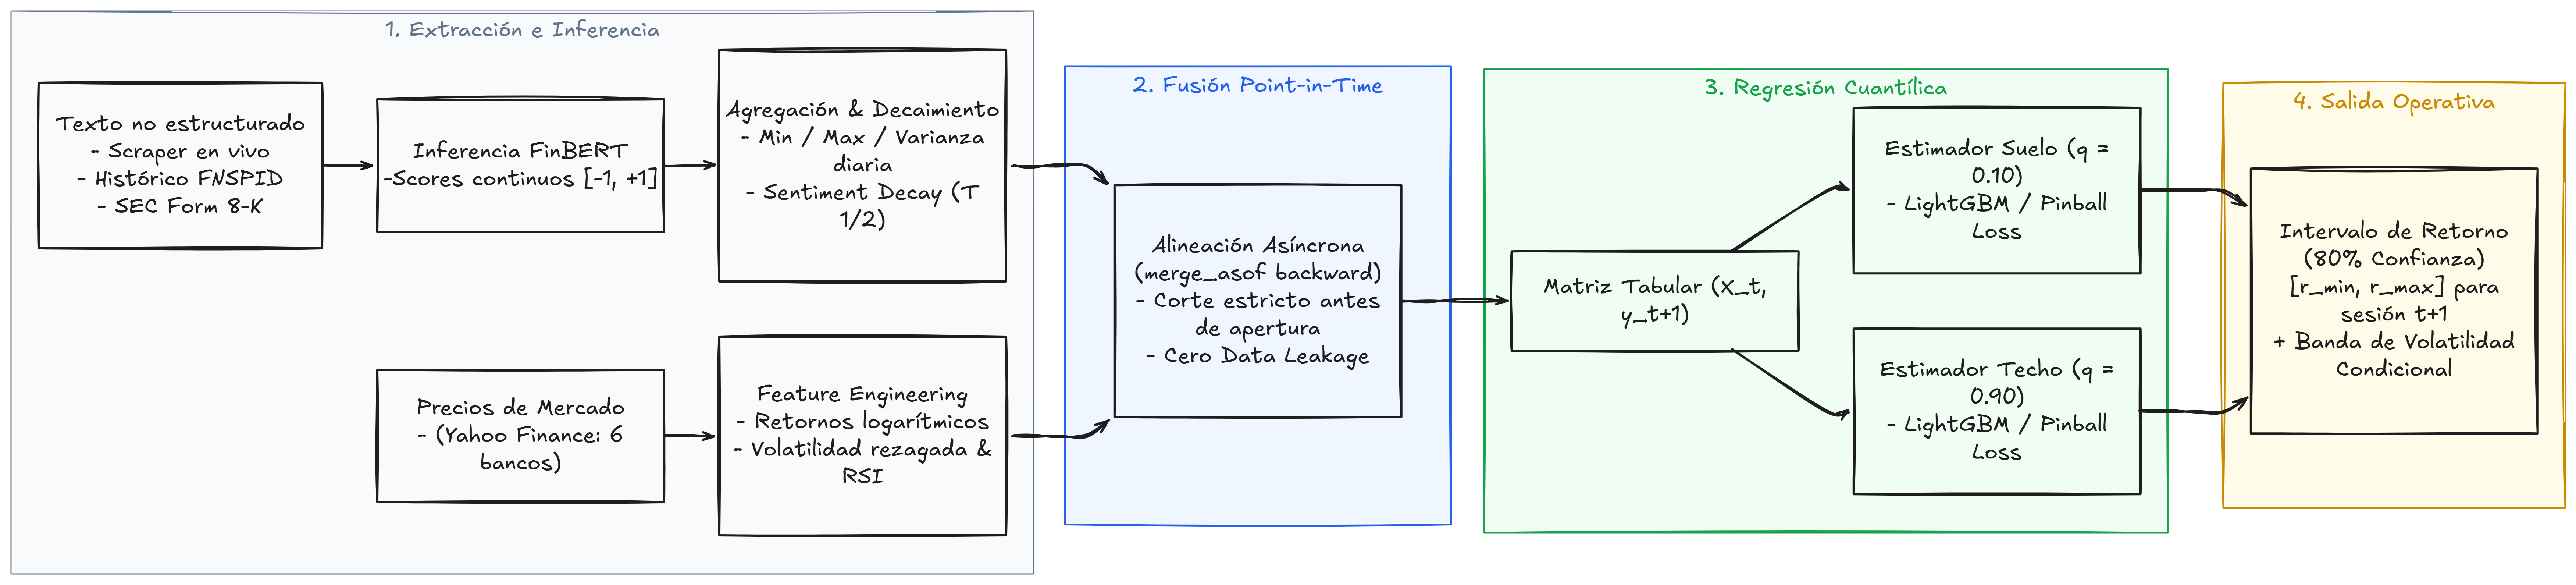
\includegraphics[width=0.95\textwidth]{diagrama-de-tfm-predecir-la-bolsa.png}
%     \caption{Arquitectura integral del flujo de datos multimodal (Bronze, Silver y Gold).}
%     \label{fig:arquitectura_medallion}
% \end{figure}

\section{Universo bancario y catálogo canónico}
La fuente única de verdad para los seis bancos del estudio reside en \texttt{src/shared/tickets.py}, centralizando \textit{tickers}, códigos CIK oficiales de la SEC y alias semánticos para evitar colisiones léxicas:

\begin{table}[H]
    \centering
    \caption{Universo bancario US Big 6 y cobertura consolidada en Capa Bronze (2010--2023).}
    \label{tab:universo_big6}
    \begin{tabular}{@{}llrr@{}}
        \toprule
        \textbf{Ticker} & \textbf{Entidad financiera} & \textbf{CIK SEC} & \textbf{Noticias Bronze} \\
        \midrule
        \texttt{JPM} & JPMorgan Chase \& Co.        & \texttt{0000019617} & 18.953 \\
        \texttt{BAC} & Bank of America Corp.        & \texttt{0000070858} & 11.509 \\
        \texttt{WFC} & Wells Fargo \& Company       & \texttt{0000072971} & 16.075 \\
        \texttt{C}   & Citigroup Inc.               & \texttt{0000831001} &  8.647 \\
        \texttt{GS}  & Goldman Sachs Group Inc.     & \texttt{0000886982} & 18.321 \\
        \texttt{MS}  & Morgan Stanley               & \texttt{0000895421} & 16.341 \\
        \midrule
        \textbf{Total} & \textbf{6 entidades} & --- & \textbf{89.846} \\
        \bottomrule
    \end{tabular}
\end{table}

\section{Fuentes de datos e ingesta multimodal (2010--2023)}
\begin{itemize}
    \item \textbf{Cotizaciones bursátiles (\texttt{src/mercado/yfinance\_extractor.py}):} Descarga histórica ajustada por \textit{splits} y dividendos (\texttt{auto\_adjust=True}) consolidada en el archivo \texttt{raw/yfinance/\allowbreak stocks\_2010\_2023.parquet}.
    \item \textbf{Eventos regulatorios SEC EDGAR (\texttt{src/sec/}):} Descubrimiento mediante API REST oficial respetando la política \textit{Fair Access} ($\le 10$ req/s). Se consolidaron tres conjuntos en R2: \texttt{8k-2010-2023.parquet} (5.424 ítems en 2.903 \textit{filings} únicos), \texttt{8k-exhibits-2010-2023.parquet} (5.531 anexos \texttt{EX-*} en 2.324 \textit{filings}, excluyendo XBRL técnicos \texttt{EX-101.*}, según ADR-007) y \texttt{10k-10q-2010-2023.parquet} (336 \textit{filings}).
    \item \textbf{Noticias financieras (\texttt{src/articulos/etl\_multisource.py}):} Procesamiento \textit{pushdown} con DuckDB sobre 21,4\,GB crudos (\textit{financial-news-multisource}), desacoplando \texttt{title} y \texttt{article}, normalizando fechas a \texttt{America/New\_York} con trazabilidad de sesión (\texttt{premarket}, \texttt{intraday}, \texttt{afterhours}, \texttt{date\_only}) y generando \texttt{raw/huggingface/multisource\_bancos\_2010\_2023.parquet} (89.846 registros tras deduplicación canónica).
\end{itemize}

\section{Diseño modular, Clean Architecture y cumplimiento normativo}
El código fuente sigue una separación estricta en capas (\textit{Dominio}, \textit{Casos de Uso/ETLs}, \textit{Infraestructura} e \textit{Inyección de Dependencias} en \texttt{src/dependencies/}), reutilizando de forma centralizada la compactación columnar en memoria (\texttt{ParquetCompactor} con PyArrow \texttt{ZSTD}) y el repositorio asíncrono S3/R2 (\texttt{S3StorageRepository}). Asimismo, el sistema cumple un diseño \textit{Compliance-by-Design} amparado en la excepción de minería de textos con fines académicos (Directiva UE 2019/790, Art.~3), inferencia efímera y ausencia total de datos personales (exención RGPD).

\chapter{Auditoría Exploratoria y Preprocesamiento (Capa Silver)}

\section{Análisis exploratorio de las fuentes Bronze}
\textit{[Completar con gráficas exportadas a \texttt{figures/} desde los notebooks \texttt{Yfinance\_2010\_2023\_EDA.ipynb}, \texttt{ExplorarDatasetsSec.ipynb} y \texttt{multisource\_financial\_news\_EDA\_2010\_2023.ipynb}: distribución anual por banco, retornos logarítmicos, colas pesadas, y predominio del Item 2.02 y anexos \texttt{EX-99.1} en los Form 8-K.]}

\section{Gatekeeper Semántico Few-Shot y poda de ruido}
La auditoría inicial de las 89.846 noticias evidenció un elevado porcentaje de contenido fuera de dominio, menciones incidentales y colisiones de subcadenas en \textit{tickers} de dos letras (\texttt{GS}, \texttt{MS}). Para evitar diluir la señal y desperdiciar cómputo en inferencia de sentimiento, se evaluó una matriz experimental $2 \times 2$ (Cross-Encoder NLI frente a Bi-Encoder; Zero-Shot frente a Few-Shot), descartando \texttt{distilbert-base-uncased-mnli} por colapso hacia categorías legales y adoptando un \textbf{Gatekeeper Prototípico Few-Shot} (\texttt{sentence-transformers/all-MiniLM-L6-v2}) en \texttt{src/articulos/models/categorizador/}.

\begin{itemize}
    \item \textbf{Centroides hiperesféricos ($\mathbb{S}^{383}$):} Representación de 7 categorías mediante prototipos canónicos e inferencia vectorial en CPU ($\sim 25\text{\,ms/doc}$).
    \item \textbf{Extracción centrada en entidad:} Ponderación adaptativa (65\,\% titular y 35\,\% fragmento relevante) mediante expresiones regulares con fronteras de palabra (\texttt{\textbackslash b}).
    \item \textbf{Reglas de desambiguación (v2):} Detección de rol de analista (\texttt{es\_rol\_analista\_tercero}), contaminación cruzada de competidor en titular y plantillas 13F/resúmenes multi-ticker. Sobre el corpus completo, la versión v2 podó el \textbf{69,71\,\% de ruido} (62.629 descartadas), conservando \textbf{27.217--27.350 artículos útiles} en capa Silver.
\end{itemize}

\section{Pipeline modular Silver y extracción de sentimiento}
La transformación hacia Silver se desacopló en tres ETLs reproducibles (\texttt{etl\_categorizador.py}, \texttt{etl\_sentimientos.py} y el orquestador \texttt{etl\_silver.py}) con cachés duales locales/R2 indexados por \texttt{cat\_hash} e \texttt{input\_hash}:

\begin{itemize}
    \item \textbf{Motor agnóstico de sentimiento (\texttt{BaseSentimentEngine}):} Define contratos estrictos en Pydantic V2 y desacopla la lógica de inferencia.
    \item \textbf{Inferencia LLM (\texttt{AnthropicSentimentEngine}):} Ejecución sobre los \textbf{27.350 artículos relevantes} alcanzando un \textbf{88,8\,\% de exactitud} frente al \textit{Ground Truth} (\texttt{v3}) con un coste total de \textbf{1,29\,USD}, auditado en \texttt{silver\_sentimientos\_eda.ipynb} junto con cruces preliminares por \texttt{category $\times$ market\_session} frente a retornos de \texttt{yfinance}.
    \item \textbf{Comparativa / Inferencia FinBERT:} \textit{[Completar con los resultados de inferencia por lotes de \texttt{ProsusAI/finbert} (polaridad continua $S = P(+) - P(-)$ y convicción $C = 1 - P(\text{Neutral})$) y comparativa de acuerdo frente al motor LLM.]}
\end{itemize}

\section{Alineación temporal Point-in-Time (Zero Data Leakage)}
\textit{[Completar: detallar el protocolo de sincronización horaria en \texttt{America/New\_York}, el corte estricto previo a la apertura de la NYSE (09:30 AM ET) mediante \texttt{pandas.merge\_asof(direction="backward")} y el tratamiento de noticias acumuladas en sesiones no hábiles.]}

\chapter{Ingeniería de Características y Modelado (Capa Gold)}

\section{Ingeniería de características cuantitativas y cualitativas}
\begin{cajadestacada}[Pendiente Fase 3]
Documentar en este apartado:
\begin{itemize}
    \item \textbf{Variables cuantitativas:} retornos logarítmicos rezagados, volatilidad móvil (\textit{rolling volatility}), RSI, medias móviles (SMA/EMA) y volumen relativo.
    \item \textbf{Variables de sentimiento y cobertura:} agregación por ventana previa a apertura respetando el desplazamiento $t+1$ de registros \texttt{date\_only}, selección de señal no colineal (\texttt{sentiment\_score} frente a probabilidades redundantes para preservar atribución en Boruta y TreeSHAP), mitigación de días sin noticias ($\ln(1+N)$, indicador \texttt{has\_news\_today}, soporte nativo de \texttt{NaN}), peso de eventos SEC 8-K y esquema de atenuación temporal ($T_{1/2}$).
\end{itemize}
\end{cajadestacada}

\section{Selección de características mediante Boruta}
Para eliminar variables ruidosas o colineales antes del entrenamiento cuantílico se emplea \textbf{Boruta}~\cite{kursa2010boruta}, un algoritmo de selección \textit{wrapper} basado en bosques aleatorios que evalúa la relevancia estadística de cada predictor frente al azar puro:
\begin{enumerate}
    \item \textbf{Variables sombra (\textit{shadow features}):} Por cada variable real $X_j$, Boruta genera una copia permutada aleatoriamente $X_j^{\text{shadow}}$ que destruye cualquier relación real con el retorno futuro $y_{t+1}$.
    \item \textbf{Contraste frente a MZSA:} Entrena un bosque aleatorio sobre el conjunto ampliado $[X, X^{\text{shadow}}]$, calcula la importancia normalizada (\textit{Z-score}) de todas las variables y fija como umbral la máxima importancia alcanzada por una sombra (\textit{Maximum Z-score among Shadow Attributes}, MZSA).
    \item \textbf{Decisión binomial iterativa:} A lo largo de múltiples iteraciones, las variables que superan significativamente a MZSA según un contraste binomial se confirman como relevantes, mientras que las que quedan por debajo se podan definitivamente.
\end{enumerate}
\textit{[PENDIENTE FASE 3 --- Documentar el listado final de variables confirmadas y rechazadas por Boruta sobre el conjunto tabular de entrenamiento sin sesgo por ticker.]}

\section{Formulación de Regresión Cuantílica (LightGBM y XGBoost)}
En lugar de estimar la esperanza condicional $E[y_{t+1} \mid X_t]$, se adopta el marco de \textbf{regresión cuantílica} de Koenker y Bassett~\cite{koenker1978quantile} mediante estimadores paralelos basados en árboles de decisión de \textbf{\textit{Gradient Boosting}} (\textit{LightGBM}~\cite{ke2017lightgbm} y \textit{XGBoost}~\cite{chen2016xgboost} con \texttt{objective='quantile'}). Internamente, ambos modelos construyen una suma aditiva $\hat{y}_q^{(M)}(x) = \sum_{m=1}^{M} \eta \, f_m(x)$ donde cada nuevo árbol $f_m$ ajusta los pseudoresiduos (gradiente negativo) de la \textbf{\textit{Pinball Loss}} para el cuantil objetivo $q \in \{0{,}10,\, 0{,}90\}$:

\begin{equation}
    \mathcal{L}_q(y, \hat{y}) = \max\Big(q(y - \hat{y}),\; (1 - q)(\hat{y} - y)\Big)
    \label{eq:pinball_loss}
\end{equation}

Mientras que \textbf{LightGBM}~\cite{ke2017lightgbm} discretiza variables continuas en histogramas y expande árboles hoja a hoja (\textit{leaf-wise}), logrando alta velocidad y captura fina de interacciones no lineales entre volatilidad y sentimiento, \textbf{XGBoost}~\cite{chen2016xgboost} crece nivel a nivel (\textit{depth-wise}) con regularización explícita $L_1/L_2$ sobre los pesos de las hojas para controlar el sobreajuste. Gracias al gradiente asimétrico de $\mathcal{L}_q$, el modelo $q=0{,}10$ penaliza nueve veces más subestimar una caída extrema que sobrestimarla, y el modelo $q=0{,}90$ hace lo inverso en subidas. Así, la amplitud del túnel predicho $\Delta_t = \hat{y}_{0.90} - \hat{y}_{0.10}$ actúa como termómetro dinámico de volatilidad e incertidumbre condicional para el día siguiente.

\section{Explicabilidad interna mediante TreeSHAP}
Para auditar qué peso real aporta cada variable técnica o textual a las bandas cuantílicas, se emplea \textbf{TreeSHAP}~\cite{lundberg2020treeshap} (\texttt{TreeExplainer}), que calcula de forma exacta los valores de Shapley de la teoría de juegos cooperativos explotando la estructura jerárquica de los árboles en tiempo polinómico $O(T L D^2)$ (siendo $T$ el número de árboles, $L$ las hojas máximas y $D$ la profundidad). Cada predicción cuantílica se descompone aditivamente como:
\begin{equation}
    \hat{y}_q(x) = \phi_0 + \sum_{j=1}^{p} \phi_j(x)
    \label{eq:treeshap}
\end{equation}
donde $\phi_0$ es el valor base esperado y $\phi_j(x)$ cuantifica la contribución marginal exacta de la característica $j$ en esa sesión bursátil.

\section{Protocolo de validación temporal y ajuste de hiperparámetros}
\textit{[PENDIENTE FASE 3 --- Documentar esquema de particionado temporal estricto (\textit{Walk-Forward} / \textit{Purged K-Fold}), prevención de fuga serial y optimización de hiperparámetros.]}

\chapter{Experimentos, Resultados y Explicabilidad}

\section{Métricas de calibración y evaluación de intervalos}
\textit{[PENDIENTE FASE 3 --- Presentar resultados fuera de muestra (\textit{out-of-sample}): cobertura empírica respecto al objetivo del 80\,\%, \textit{Pinball Loss} medio y \textit{Winkler Score} por entidad bancaria.]}

\section{Estudio de ablación: modelo cuantitativo puro frente a híbrido}
\textit{[PENDIENTE FASE 3 --- Comparativa controlada entre LightGBM/XGBoost entrenado solo con indicadores de mercado frente al modelo multimodal enriquecido con sentimiento de noticias y eventos SEC 8-K.]}

\section{Explicabilidad mediante TreeSHAP}
\textit{[PENDIENTE FASE 3 --- Análisis global (\textit{beeswarm} / importancia media $|SHAP|$) y casos locales de eventos de alta volatilidad para auditar qué peso aporta la señal textual frente a las métricas técnicas.]}

\section{Simulación de gestión de riesgo (Backtesting)}
\textit{[PENDIENTE FASE 3 --- Evaluación de una estrategia de dimensionamiento de posición y cobertura dinámica condicionada a la amplitud del túnel cuantílico frente a la referencia pasiva \textit{Buy \& Hold} (Sharpe, Drawdown máximo, volatilidad realizada).]}

\chapter{Despliegue, Calidad y Visualización}

\section{Arquitectura de orquestación e inferencia diaria}
\textit{[PENDIENTE FASE 4 --- Documentar la orquestación diaria programada previa a la apertura de mercado (Apache Airflow a las 08:30 AM ET) y la ejecución \textit{serverless} en AWS Lambda (\texttt{python:3.13-slim}) leyendo/escribiendo sobre Cloudflare R2.]}

\section{Aseguramiento de la calidad del software (QA)}
Para garantizar reproducibilidad y mantenibilidad industrial en el desarrollo colaborativo, el repositorio incorpora:
\begin{itemize}
    \item \textbf{Gestión determinista:} Entorno gestionado íntegramente con \texttt{uv} (\texttt{pyproject.toml} + \texttt{uv.lock}) sobre Python 3.14.
    \item \textbf{Pruebas automatizadas:} Suite unitaria y de integración con \texttt{pytest}, \texttt{pytest-asyncio} y \texttt{moto} (simulación en memoria de S3 sin depender de credenciales reales), superando los \textbf{126 tests aprobados}.
    \item \textbf{Integración continua y análisis estático:} Pipeline en GitHub Actions (\texttt{pr\_validation.yml}) con verificación de \texttt{ruff} y puerta de calidad en \textbf{SonarCloud}.
\end{itemize}

\section{Cuadro de mando operativo (Streamlit Community Cloud)}
\textit{[PENDIENTE FASE 4 --- Documentar el diseño e implementación del dashboard de solo lectura sobre los Parquet Gold en Cloudflare R2: visualización del túnel cuantílico del 80\,\%, termómetro de volatilidad condicional, titulares filtrados y explicaciones TreeSHAP por ticker.]}

\chapter{Conclusiones, Impacto y Líneas Futuras}

\section{Síntesis de hallazgos y cumplimiento de objetivos}
\textit{[PENDIENTE FASE 4 --- Valorar de forma crítica el grado de cumplimiento de los objetivos específicos OE1--OE5, validando o matizando las hipótesis iniciales sobre el poder informativo del sentimiento pre-apertura en el sector bancario estadounidense.]}

\section{Análisis de impacto operativo y retorno de inversión (ROI)}
\textit{[PENDIENTE FASE 4 (Requisito explícito de EBIS) --- Traducir las métricas estadísticas del modelo y el coste operativo nulo de la arquitectura (\textit{Always Free}) a valor de negocio para mesas de tesorería, gestión de carteras o sistemas \textit{Robo-Advisor}: reducción de exposición ante eventos de cola, dimensionamiento dinámico del riesgo y ahorro frente a proveedores comerciales de datos y APIs.]}

\section{Limitaciones del estudio}
\textit{[Completar: limitaciones observadas en cobertura histórica de prensa, latencia de publicación de anexos SEC, restricciones de cómputo sin GPU dedicada en producción, etc.]}

\section{Líneas futuras de trabajo}
\begin{itemize}
    \item Extensión del universo de estudio hacia otros sectores sistémicos (tecnología, energía) o índices europeos.
    \item Incorporación de datos macroeconómicos de alta frecuencia (FRED) y análisis específico de los anexos \texttt{EX-99.1} e informes trimestrales \texttt{10-Q/10-K}.
    \item Integración en tiempo real de ingesta continua mediante el motor de \textit{Web Scraping} distribuido y calibración conformal de intervalos (\textit{Conformalized Quantile Regression}).
\end{itemize}


% ==============================================================================
% BIBLIOGRAFÍA Y ANEXOS
% ==============================================================================
\printbibliography[heading=bibintoc, title={Referencias bibliográficas}]

\appendix
\chapter{Registro de Decisiones Arquitectónicas (ADRs)}

Como respaldo de ingeniería al cuerpo principal de la memoria, se resumen las decisiones técnicas críticas adoptadas durante el ciclo de vida del proyecto:

\begin{table}[H]
    \centering
    \caption{Resumen de Architecture Decision Records (ADRs) del proyecto.}
    \label{tab:adrs_resumen}
    \begin{tabularx}{\textwidth}{@{}l >{\raggedright\arraybackslash}p{4.3cm} >{\raggedright\arraybackslash}X@{}}
        \toprule
        \textbf{ID} & \textbf{Decisión clave} & \textbf{Justificación técnica y consecuencia} \\
        \midrule
        ADR-001 & Cloudflare R2 frente a AWS S3 & API S3 v4 compatible con 0\,€ en \textit{egress} y capa gratuita perpetua de 10\,GB. \\
        ADR-002 & FinBERT frente a LLM genéricos & Inferencia determinista local en CPU sin latencia ni coste por token en producción. \\
        ADR-003 & Regresión cuantílica frente a clasificación & Estimación de intervalo al 80\,\% $[y_{0.10}, y_{0.90}]$ como medida directa de riesgo condicional. \\
        ADR-004 & Alineación \texttt{merge\_asof} hacia atrás & Erradicación formal de \textit{Look-Ahead Bias} respecto al corte de apertura NYSE. \\
        ADR-005 & Gatekeeper Few-Shot (\texttt{all-MiniLM-L6-v2}) & Poda del 69,71\,\% de ruido (v2) en $\sim 25\text{\,ms/doc}$ frente al colapso multiclase de NLI. \\
        ADR-006 & Estándar KISS \& DRY en infraestructura & Reutilización estricta de \texttt{ParquetCompactor} y \texttt{S3StorageRepository} evitando fugas de conexión. \\
        ADR-007 & Parquet desacoplado para anexos 8-K & Almacenamiento separado de 5.531 \texttt{EX-*} enlazados por \texttt{accession\_number} sin romper esquemas previos. \\
        \bottomrule
    \end{tabularx}
\end{table}

\chapter{Esquemas de Datos y Reproducción del Entorno}

\section{Catálogo de conjuntos de datos en Cloudflare R2}
\textit{[Completar al cierre de Fase 3 con el esquema exacto de columnas y tipos de las capas Bronze, Silver y Gold.]}

\section{Guía rápida de reproducción}
El entorno completo del proyecto se reproduce de forma determinista mediante \texttt{uv}:

\begin{lstlisting}
# Clonar repositorio e instalar dependencias exactas
git clone https://github.com/ArturoCarrilloJimenez/TFM-Master.git
cd TFM-Master
uv sync

# Ejecutar la suite completa de pruebas unitarias
uv run pytest src/test/ --cov=src --cov-report=term-missing
\end{lstlisting}


\end{document}
